% !TEX program = pdflatex
% !TEX ext =  --interaction=nonstopmode --enable-etex --enable-write18
% !BIB program = biber
%%%==============================================================================
%% Copyright 2022-23 by Alceu Frigeri
%%
%% Document (sample) file using the class ufrgscca
%%
%% This file was adapted from:
%% Meta-monografia de exemplo genérico de uso da classe delaetex.cls
%% Copyright (C) 2004..2016 Walter Fetter Lages <fetter@ece.ufrgs.br>
%%
%%%==============================================================================
%\documentclass[repeatfields,openright,overleaf,nomicrotype]{ufrgscca}
\documentclass[repeatfields,xlists,xpacks,oneside]{ufrgscca}

\addbibresource{modeloTCC.bib}
\usepackage{float}

%%%%%%%%%%%%%%%%%%%%%%
%%%%%%%%%%%%%%%%%%%%%%
%%
%% TCC Class options
%%
%% english   => paper/report in english
%%     \documentclass[english]{tcc}
%%
%% repeatfields => (abnt) references with same authors have their names repeated.
%%												otherwise only the first reference of them will be printed.
%%     \documentclass[repeatfields]{tcc}
%%
%% openright => force the start of a chapter at odd pages.
%%     \documentclass[openright]{tcc}
%%
%% oneside => single side document
%%     \documentclass[oneside]{tcc}
%%
%% NOTE : openright, oneside :: IF you are going to print the doc, single sided, the best is to just use
%%                              the [oneside] option.
%%                              IF you are going to print the doc, double sided, the best is to just use the
%%                              the [openright] option.
%%
%% relnum => figures/tables counters are reset with each chapter.
%%     \documentclass[relnum]{tcc}
%%
%% showframe => (for drafts only) auxiliary visual guide to page frame.
%%     \documentclass[showframe]{tcc}
%%
%% showlabels =>  (for drafts only) prints labes/citeref strings on the side bar.
%%     \documentclass[showlabels]{tcc}
%%
%%
%%%%%%%%%%%%%%%%%%%%%%
%%%%%%%%%%%%%%%%%%%%%%

%
% inicio do documento
%

\begin{document}



%%%%%%%%%%%%%%%%%%%%%%
%%%%%%%%%%%%%%%%%%%%%%
%%
%% \MakeCoverPages produz as páginas iniciais
%% as opções são
%%
%% tccI => para TCC-I
%% tccII => para TCC-II
%% internship => para Estágio Obrigatório
%% internship-opt => para Estágio Não Obrigatório
%% class-report => para relatórios/trabalhos de uma disciplina
%%
%%%%%%%%%%%%%%%%%%%%%%
%%%%%%%%%%%%%%%%%%%%%%

%\MakeCoverPages{tccI}
\MakeCoverPages{tccII}

% palavras-chave
% iniciar todas com letras minúsculas, exceto no caso de abreviaturas
%
\mainkeywords{Transferência de energia sem fio}
\mainkeywords{Cápsula de endoscopia}
\mainkeywords{Transmissão de dados}
\mainkeywords{Validação de sistemas}


% resumo no idioma do documento
\begin{mainabstract}

Este trabalho apresenta a implementação e a validação prática de um sistema de captura, processamento básico, transmissão e reconstrução de imagens destinado ao desenvolvimento de uma cápsula endoscópica sem fio. O estudo dá continuidade à etapa conceitual anteriormente desenvolvida, avançando para a construção de um protótipo funcional em bancada que integra câmera, microcontrolador e enlace RF de baixa potência. A arquitetura proposta utiliza uma câmera CMOS OV7670, microcontroladores de baixo custo e o transceptor NRF24L01+, permitindo avaliar, de forma quantitativa, o desempenho do pipeline completo de aquisição e transmissão de dados. São conduzidos testes de leitura direta da câmera, validação do protocolo lógico de empacotamento, transmissão sem fio e aplicação de compressão RLE para redução de banda. Os resultados demonstram estabilidade do enlace, reconstrução consistente dos quadros e aumento significativo na taxa de transmissão quando a compressão é aplicada. O trabalho estabelece, assim, uma base experimental sólida para o aprimoramento futuro do sistema por meio da adoção de algoritmos de compressão mais eficientes, microcontroladores com maior capacidade de processamento e integração com o sistema de transferência de energia sem fio previsto no desenvolvimento completo da cápsula.

\end{mainabstract}

% resumo no outro idioma
% como parametro devem ser passadas as palavras-chave
% no outro idioma, separadas por vírgulas

%%
%% No caso do documento ser em ingles, usar
%%  \begin{otherabstract}[brazilian]
%%
\begin{otherabstract}

\otherkeywords{Wireless Power Transfer}
\otherkeywords{Endoscopic Capsule}
\otherkeywords{Data Transmission}
\otherkeywords{System Validation}

This work presents the implementation and practical validation of an image capture, basic processing, transmission, and reconstruction system designed for a wireless endoscopic capsule. The study extends the conceptual foundation previously developed, advancing toward the construction of a functional bench prototype that integrates a CMOS camera, a microcontroller, and a low-power RF communication link. The proposed architecture employs an OV7670 image sensor, low-cost microcontrollers, and the NRF24L01+ transceiver, enabling a quantitative evaluation of the complete acquisition and transmission pipeline. Tests include raw camera data acquisition, verification of the logical packetization protocol, wireless transmission, and the application of Run-Length Encoding (RLE) to reduce bandwidth usage. The results demonstrate a stable RF link, consistent frame reconstruction, and a significant increase in throughput when compression is applied. The study thus provides a solid experimental foundation for future improvements, including the adoption of more efficient compression algorithms, higher-performance microcontrollers, and integration with the wireless power transfer system envisioned for the full capsule design.

\end{otherabstract}


% sumario
\setcounter{tocdepth}{3}

% lista de ilustrações
\listoffigures

% lista de tabelas
\listoftables

% lista de listagens (código fonte)
%\listofcodelist %% doesn't work on overleaf

% lista de abreviaturas e siglas
% o parametro deve ser a abreviatura mais longa
\begin{listofabbrv}{PPGEE}
	\item[WCE] Wireless Capsule Endoscopy (Endoscopia por Cápsula Sem Fio)
	\item[WPT] Wireless Power Transfer (Transmissão de Energia Sem Fio)
	\item[RC] Receiving Coil (Bobina de Recepção)
	\item[CMOS] Complementary Metal-Oxide-Semiconductor (Semicondutor de Óxido Metálico Complementar)
	\item[RF] Radio Frequency (Frequência de Rádio)
	\item[IMU] Inertial Measurement Unit (Unidade de Medição Inercial)
           \item[DVP] Digital Video Port (Porta Digital de Vídeo)
	\item[VSYNC] Vertical Synchronization (Sincronismo Vertical)
	\item[HREF] Horizontal Reference (Referência Horizontal)
	\item[PCLK] Pixel Clock (Clock de Pixel)
	\item[WLI] White Light Imaging (Imagem por Luz Branca)
	\item[RLE] Run-Length Encoding (Codificação por Comprimento de Execução)
	\item[DPCM] Differential Pulse Code Modulation (Modulação por Código de Pulso Diferencial)
	\item[FPS] Frames Per Second (Quadros por Segundo)
	\item[CRC] Cyclic Redundancy Check (Verificação de Redundância Cíclica)
	\item[SPI] Serial Peripheral Interface (Interface Serial de Periféricos)
	\item[I2C] Inter-Integrated Circuit (Barramento Interintegrado)

\end{listofabbrv}

% lista de símbolos é opcional
%\begin{listofsymbols}{$\alpha\beta\pi\omega$}
%       \item[$\sum$] Somatório
%       \item[$\alpha\beta\pi\omega$] Fator de inconstância do resultado
%\end{listofsymbols}


\tableofcontents


% AQUI COMEÇA O TEXTO PROPRIAMENTE DITO

% introducao
\chapter{Introdução}

A endoscopia por cápsula sem fio (WCE) tem recebido muita atenção como uma alternativa útil à endoscopia tradicional, na qual o método de diagnóstico comum para lesões gástricas envolve a passagem de um tubo longo e flexível equipado com uma câmera de vídeo pela garganta do paciente. Além disso, a endoscopia tradicional é realizada sob sedação podendo causar eventos adversos em pacientes de alto risco \cite{amornyotin2013sedation}, como aqueles com doenças cardíacas e pulmonares graves ou pacientes idosos.

A WCE tornou-se um dispositivo de diagnóstico preferido para doenças do trato gastrointestinal desde sua invenção devido às suas características não invasivas e indolores \cite{iddan2000wireless}, especificamente para a mucosa do intestino delgado \cite{pennazio2004outcome}, que não podia ser alcançada por endoscópios convencionais \cite{pennazio2004outcome}. Ao engolir uma cápsula do tamanho de um comprimido, anormalidades gástricas como pólipos, úlceras, sangramento e infecções podem ser detectadas e diagnosticadas através da transmissão de vídeo sem fio \cite{khan2020computer}.

Para melhorar a qualidade do diagnóstico, várias especificações importantes da WCE, como resolução de imagem, taxa de quadros e tempo de operação, precisam de melhorias, o que consumirá mais energia \cite{basar2014application}. No futuro, as cápsulas não se limitarão apenas à detecção de imagens, mas também envolverão múltiplas tarefas (por exemplo, biópsia, liberação de medicamentos e movimentos autônomos) \cite{meng2021novel}. Essas funções adicionais aumentarão o consumo de energia, que a bateria convencional não consegue satisfazer. Consequentemente, o fornecimento de energia para WCEs tem sido uma questão desafiadora, pois a cápsula é muito pequena para transportar uma bateria de grande capacidade e um fio de alimentação pode causar desconforto aos pacientes ou restringir o movimento da cápsula \cite{gao2022stable}. Nesse contexto a transmissão de energia sem fio (WPT) baseada em acoplamento indutivo é uma solução promissora para resolver a questão energética dos WCEs.

O design dos sistemas que compõem a WCE envolve a integração de várias tecnologias para garantir a operação eficiente e a coleta precisa de dados. O sistema de WPT permite que a cápsula receba energia de uma bobina transmissora, independentemente de sua orientação no trato gastrointestinal, utilizando acoplamento indutivo \cite{kim2021capsule}. A cápsula em si é equipada com um conjunto de bobinas receptoras, uma unidade de medição inercial (IMU) para determinar sua orientação, e componentes eletrônicos como câmeras, baterias e LEDs \cite{zhang2024transmitter}. Esses elementos trabalham em conjunto para fornecer energia e coletar dados de imagem, transmitindo informações em tempo real para fora do corpo.

O presente trabalho dá continuidade ao estudo desenvolvido em \textcite{murliky2021study}, que propôs estratégias de controle para estabilidade da transmissão de energia sem fio em aplicações de endoscopia. Enquanto o estudo anterior concentrou-se na análise teórica do link indutivo e na caracterização de um protótipo contendo apenas o sistema de recepção de energia, este trabalho propõe a implementação prática e validação experimental dos subsistemas eletrônicos fundamentais de uma cápsula endoscópica. São abordadas a captura de imagem com sensores CMOS, o processamento embarcado mínimo necessário para segmentação e organização dos dados, a compressão simples por RLE, o empacotamento lógico dos quadros, a transmissão sem fio com módulos NRF24L01+ e a reconstrução completa das imagens no receptor. O foco passa a ser a construção de uma prova de conceito funcional, estruturada de forma modular, que permita validar individualmente cada subsistema e estabelecer uma base técnica sólida para futuras versões miniaturizadas e para a incorporação de algoritmos de compressão mais avançados e microcontroladores de maior desempenho.

%\subsection{Objetivos Específicos}

%\begin{enumerate}[tcc,alpha)]
%\item Validar os subsistemas da cápsula endoscópica por meio de testes práticos e análises para assegurar seu funcionamento adequado e integração eficiente.
%\item Projetar o sistema de forma modularizada, permitindo a validação independente dos subsistemas, incluindo recepção de energia sem fio, captura de dados de imagem, processamento de dados e transmissão.
%\item Validar o subsistema de recepção de energia sem fio, que engloba a retificação e os reguladores de tensão, garantindo que a cápsula receba energia de forma eficiente e estável.
%\item Realizar testes de desempenho para os sistemas de captura de dados de imagem, processamento de dados e transmissão, assegurando a qualidade das imagens, a eficácia do processamento e a integridade da transmissão de dados.
%\end{enumerate}

%%%%%%%%%%%%%%% REVISAO BIBLIOGRAFICA %%%%%%%%%%%%%%%

% Revisão bibliográfica (2 paginas)
\chapter{Revisão bibliográfica}
%estado da arte do problema/solução apresentada na literatura (2 paginas)
Este capítulo oferece uma revisão sobre a tecnologia de cápsulas endoscópicas, destacando as principais inovações em desenvolvimento, desafios e soluções encontradas na literatura científica. Serão abordados alguns aspectos sobre as tecnologias de transmissão de energia sem fio, e os sistemas que englobam a captura e transmissão de dados, além dos desafios e limitações atuais.

\section{Cápsulas Endoscópicas}


O mercado de endoscopia por cápsula sem fio (WCE) tem atraído crescente interesse industrial e acadêmico. O primeiro sistema comercial, a PillCam, foi desenvolvido pela Given Imaging em 2000 \cite{Pillcam} e aprovado pela \textit{Food and Drug Administration} (FDA) em 2001 para diagnóstico do esôfago, intestino delgado e cólon, consolidando-se como o modelo comercial de maior adoção.

Na literatura, diversos trabalhos descrevem protótipos baseados em FPGA (\textit{Field-Programmable Gate Arrays}). Em \textcite{cavallotti2011fpga}, é apresentado um sistema de desenvolvimento para validação da eletrônica da cápsula, com compressão DCT e armazenamento em SRAM externa. Em \textcite{covi2010miniaturized}, um dispositivo com fio que integra sensor CMOS e placa programável foi avaliado em testes \textit{ex-vivo} e \textit{in-vivo}. Já em \textcite{meng2021novel}, um protótipo com múltiplas câmeras, FPGA e memória flash armazena os dados localmente, ao custo de menor praticidade na recuperação das imagens.

Também são reportados sistemas baseados em microcontroladores e componentes comerciais. Em \textcite{gao2022stable}, descreve-se um protótipo simples com câmera CMOS analógica, modulador RF e iluminação por LEDs brancos. O trabalho de \textcite{khan2020computer} apresenta uma cápsula baseada em microprocessadores ARM e Linux embarcado, utilizando sensor CCD digital e compressão JPEG2000. Em \textcite{cheng2010novel}, é descrita uma cápsula que integra sensor CMOS com compressão JPEG embarcada, microcontrolador ARM Cortex-M3 e transceptor RF.

De modo geral, cápsulas alimentadas por energia sem fio raramente exploram arquiteturas de bobinas receptoras em quadratura, que poderiam aumentar a robustez do acoplamento indutivo em diferentes orientações da cápsula. Do ponto de vista de imagem, a maioria dos dispositivos comerciais limita-se à captura por luz branca (WLI), com pouca flexibilidade para modalidades alternativas ou processamento avançado. Esses aspectos evidenciam limitações recorrentes tanto no subsistema de energia quanto no de aquisição de imagem. A Figura \ref{fig:exemplos-capsulas} apresenta exemplos de cápsulas citadas na literatura. Nesse contexto, torna-se relevante o desenvolvimento de uma arquitetura modular e programável, que permita investigar diferentes estratégias de alimentação e algoritmos de imagem, preservando a possibilidade de miniaturização futura.

\begin{figure}[htbp]
  \centering
  \caption{Exemplos de cápsulas endoscópicas existentes incluem: (a) um protótipo desenvolvido em um estudo utilizando FPGA e bateria não recarregável; (b) um protótipo de WCE com bateria recarregável; e (c) o modelo comercial PillCam ESO 2.}
  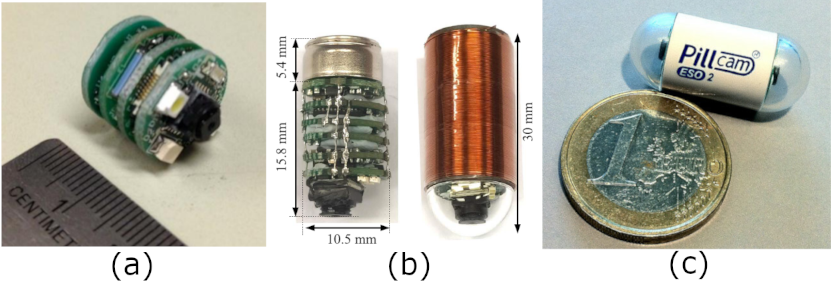
\includegraphics[width=0.6\textwidth]{images/exemplos-capsulas.png}\\
  \label{fig:exemplos-capsulas}
  \sourcecitation{Elaborada pelo autor a partir de \cite{khan2013capsule}, \cite{zhang2024transmitter} e \cite{Pillcam}.}
\end{figure}

\section{Desafios e Limitações Atuais}
Apesar dos avanços significativos, ainda existem desafios notáveis. A demanda energética para a WCE continua sendo um obstáculo, aumentando com a qualidade da imagem e recursos avançados incorporados. A cápsula mais básica requer cerca de 30 mW de energia para alimentar um sensor de imagem CMOS, LEDs e transceptor RF \cite{xie2006micro}. Cápsulas de vídeo de alta resolução (HRVCs) utilizam dispositivos de imagem de maior resolução, maior intensidade de luz e maior largura de banda de transmissão RF, exigindo até 200 mW \cite{pan2011video}. A próxima geração, conhecida como cápsulas robóticas (RCEs), incluirá sistemas avançados de controle, locomoção, foco automático, compressão de imagem e outros sensores, demandando até 400 mW \cite{carta2010wireless}. Cápsulas multifuncionais (MMR) podem exigir até 570 mW \cite{ye2008development}. A capacidade das baterias atuais é insuficiente, portanto, sistemas de WPT são necessários para atender a essa demanda com eficiência, estabilidade, segurança e portabilidade A Figura \ref{fig:power-requirement-wce} ilustra o consumo energético para diferentes modelos de cápsulas.

\begin{figure}[htbp]
  \centering
  \caption{Requisito de energia para diferentes modelos de WCE.}
  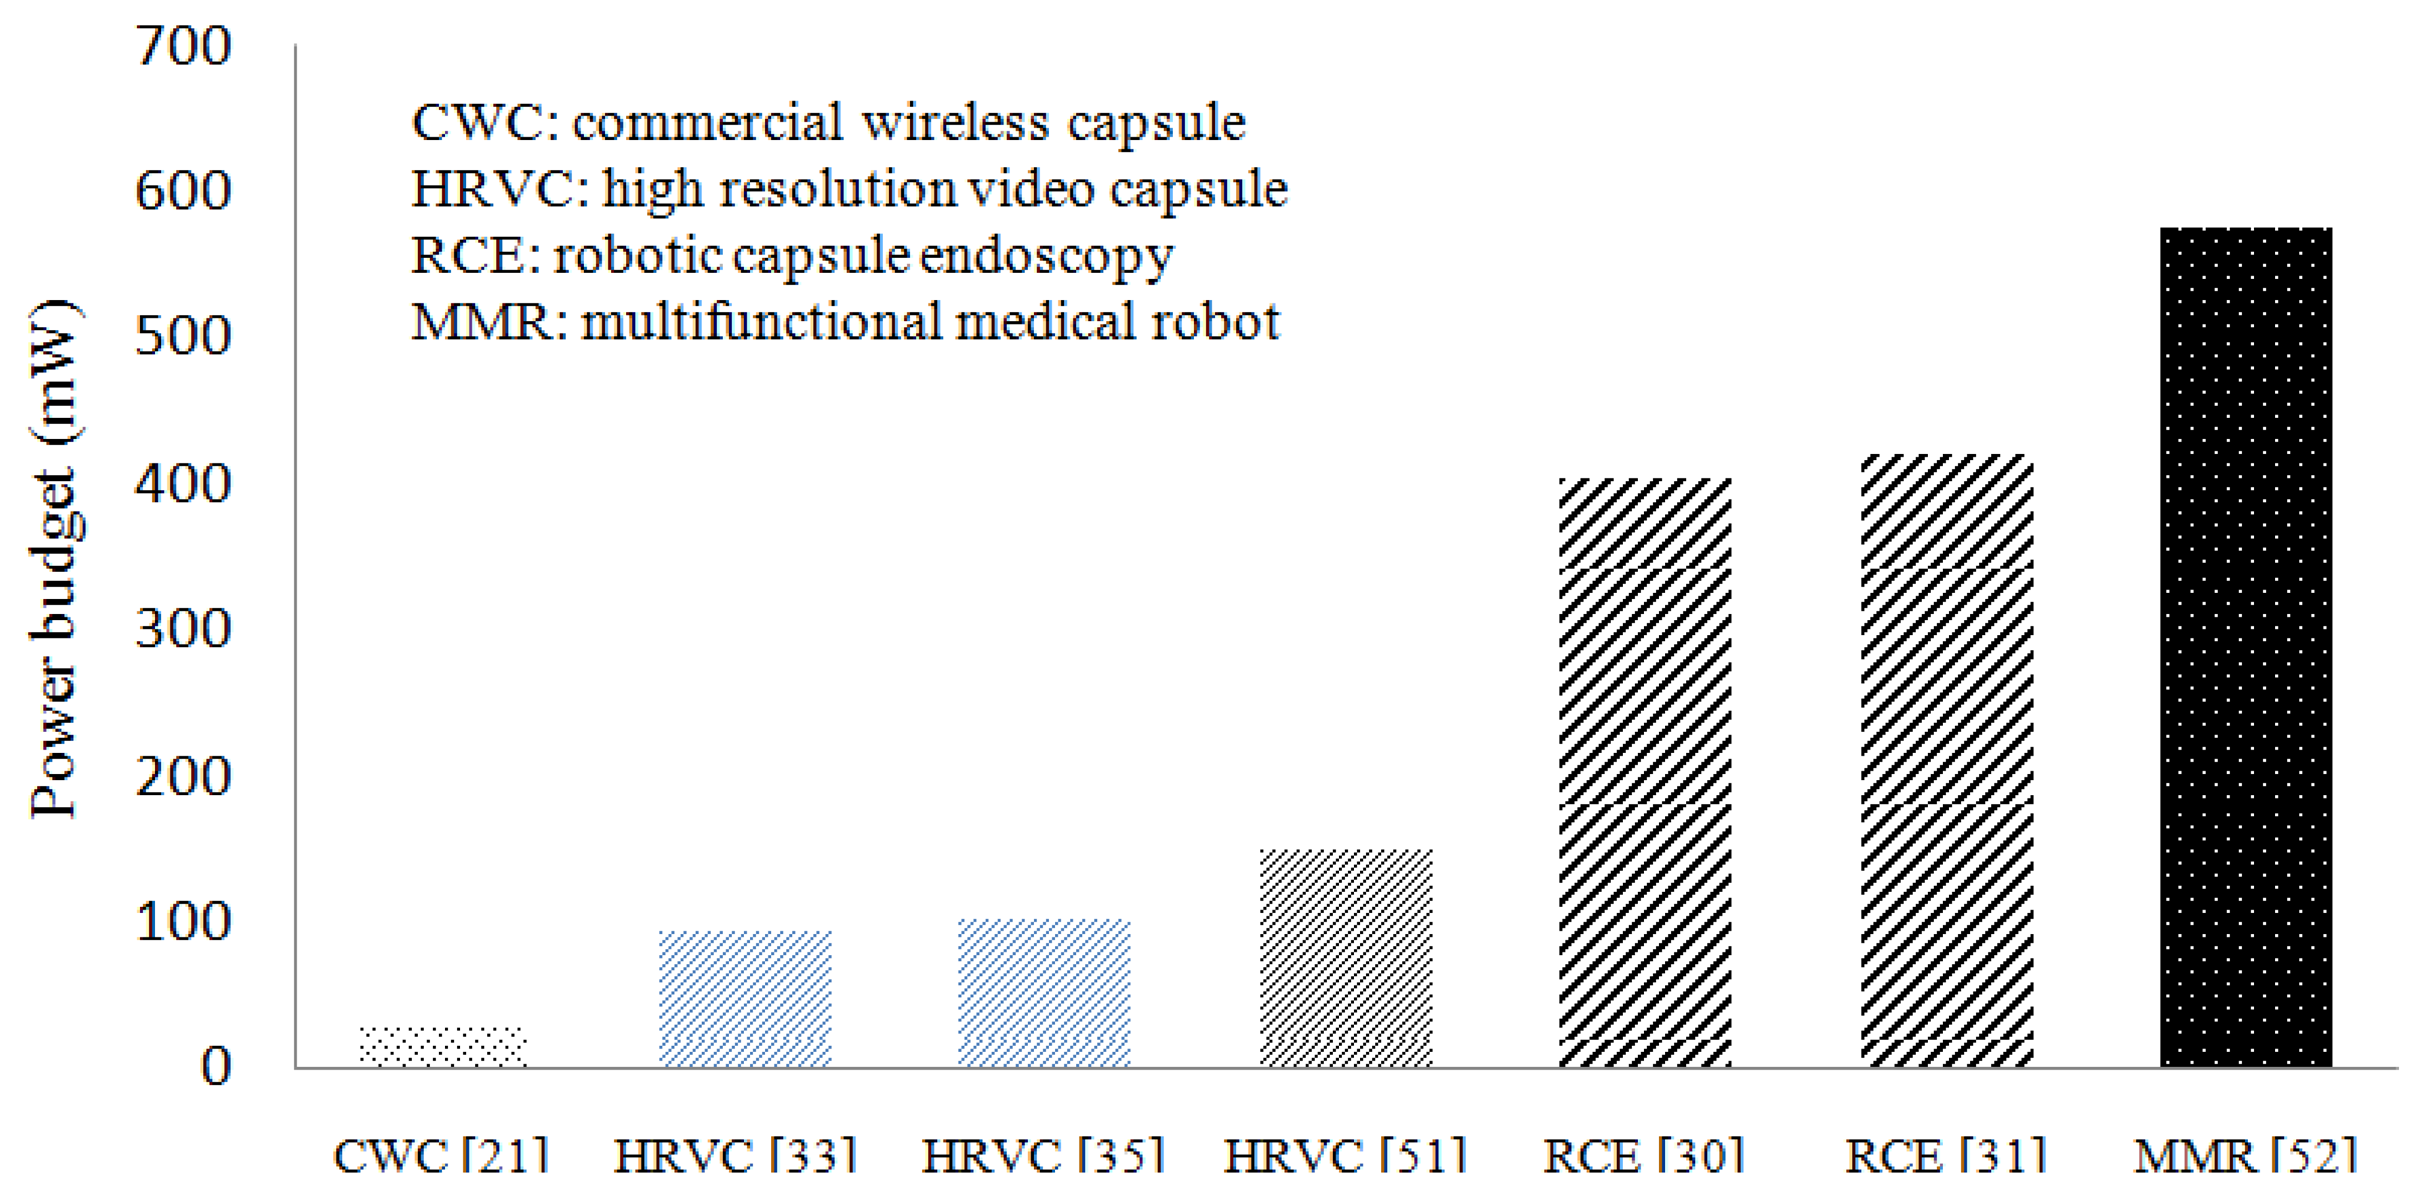
\includegraphics[width=0.5\textwidth]{images/power-requirement-wce.png}\\
  \label{fig:power-requirement-wce}
  \sourcecitation{\cite{basar2014application}}
\end{figure}


%%%%%%%%%%%%%%% FUNDAMENTAÇÂO TEORICA %%%%%%%%%%%%%%%

% embasamento téorico para o desenvolvimento da solução proposta (até 10 paginas)
\chapter{Fundamentação teórica}

Este capítulo apresenta a fundamentação necessária para compreender os elementos centrais do presente trabalho. A intenção é condensar, com linguagem técnica e rigor acadêmico, os conceitos que embasam a proposta: limites energéticos e alternativas de alimentação, características dos sensores de imagem em miniatura, restrições e estratégias de processamento embarcado, técnicas de compressão adequadas a plataformas com recursos limitados e aspectos do enlace RF utilizado na validação experimental. As seções seguintes desenvolvem esses tópicos de forma integrada, sustentando as decisões metodológicas das partes experimentais.

\section{Transferência de energia para cápsulas endoscópicas - visão geral}

Nesta seção apresenta-se, de forma concisa, os princípios físicos e as implicações de projeto associados à transferência de energia sem fio (Wireless Power Transfer — WPT) aplicadas a cápsulas endoscópicas, bem como os efeitos dessas escolhas no orçamento energético do dispositivo.

A alimentação de cápsulas endoscópicas constitui uma restrição projetual crítica: o reduzido volume interno limita a capacidade de armazenamento de energia e, simultaneamente, sensores, iluminação e transmissão impõem demandas periódicas significativas. Entre as técnicas de WPT, o acoplamento indutivo é a abordagem mais adotada em protótipos biomédicos por permitir transferência de potência em curta distância com eficiência compatível às necessidades clínicas. O fenômeno físico subjacente é a indução magnética entre bobinas transmissora e receptora; a potência acoplada depende do fator de acoplamento, das perdas ôhmicas, do fator de qualidade das bobinas e da adequação do circuito de ressonância e da etapa de retificação no receptor. Trabalhos de referência descrevem modelagens e técnicas de compensação que visam manter a potência entregue estável frente a variações de acoplamento e orientação. \cite{motta2016transmissao,murliky2017multivariable}

A engenharia do subsistema de energia exige análise integrada: estima-se a potência disponível na bobina receptora, aplica-se uma estimativa das perdas no retificador e nos reguladores e, a partir daí, define-se um orçamento por subsistema (câmera, LEDs, processamento, transmissor RF). Em protótipos e estudos de bancada, a captura de imagem e o arranjo de iluminação costumam consumir dezenas de miliwatts em operação contínua; a transmissão RF pode aumentar esse consumo dependendo da taxa de dados e do tempo de transmissão efetivo, forçando trade-offs entre resolução, taxa de quadros (FPS) e autonomia operacional \cite{pan2011video,basar2014application}. A Figura \ref{fig:sistema-endoscopia-capsula} ilustra um arranjo típico empregado na literatura, no qual uma bobina transmissora externa energiza a cápsula equipada com múltiplas bobinas receptoras dispostas em quadratura. Essa configuração reduz a sensibilidade à orientação do dispositivo durante sua movimentação natural no trato gastrointestinal, mitigando oscilações de potência recebida e contribuindo para a estabilidade do sistema de alimentação \cite{murliky2022tracking}.

\begin{figure}[htbp]
  \centering
  \caption{Sistema de endoscopia com bobina transmissora externa e detalhe da cápsula de endoscopia com três bobinas receptoras em quadratura.}
  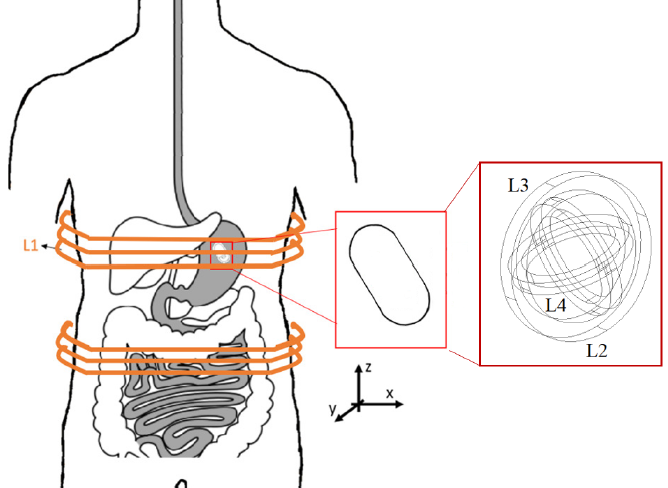
\includegraphics[width=0.55\textwidth]{images/sistema-endoscopia-capsula0.png}\\
  \label{fig:sistema-endoscopia-capsula}
  \sourcecitation{\cite{murliky2022tracking}}
\end{figure}

Além das métricas médias, um projeto de WPT deve considerar variáveis dinâmicas: deslocamento e rotação da cápsula no trato gastrointestinal, variação da impedância vista pela bobina receptora e requisitos de segurança eletromagnética. Em estágio conceitual, modelagens do link indutivo e estimativas de margens de eficiência servem para definir limites aceitáveis de consumo, tanto para operação alimentada por WPT quanto para casos híbridos com bateria suplementar \cite{motta2016transmissao}.

\section{Eletrônica de aquisição de imagens}

Esta seção descreve os princípios de operação de sensores de imagem miniaturizados usados em cápsulas e os elementos de controle e sincronização que condicionam a aquisição e o fluxo de dados.

\subsection{Sensores de imagem: arquitetura e características}

Sensores compactos empregados em aplicações médicas geralmente adotam arquitetura CMOS integrada, que reúne matriz de fotodetectores, circuitos de leitura e periféricos de controle. Esses sensores expõem, tipicamente, uma interface paralela conhecida como Digital Video Port (DVP), composta por linhas de dados (por exemplo D0..D7), sinais de sincronismo (VSYNC, HREF) e o clock de pixel (PCLK). A saída via DVP permite leitura síncrona com PCLK: a cada borda válida de PCLK um novo byte (ou nibble, conforme modo) pode ser lido, VSYNC sinaliza início/fim de quadro e HREF delimita os intervalos ativos de cada linha. A configuração fina do sensor — seleção do formato de saída, habilitação de AEC/AGC, ajuste de ganho, controle de exposição e outros parâmetros — é realizada por uma interface de controle serial (normalmente I\textsuperscript{2}C ou o protocolo SCCB proprietário), que escreve e lê registradores internos do sensor \cite{cavallotti2011fpga,meng2021novel}.

A escolha do formato de saída impacta diretamente o volume de dados e a complexidade de processamento: formatos como RGB565 implicam dois bytes por pixel; formatos YUV422 transmitem amostras de crominância intercaladas com luminância e permitem extrair apenas a componente Y (luminância) quando o interesse é em imagens em tons de cinza, reduzindo o volume útil. Quando o sensor não possui memória FIFO interna, o host é responsável por capturar os dados no ritmo imposto por PCLK, o que exige leitura síncrona em modo `streaming' e impõe restrições de latência e de tamanho de buffer no firmware. A compatibilidade entre formato de pixel, capacidade de leitura e recursos de memória do processador é, portanto, um ponto decisivo de projeto \cite{cavallotti2011fpga}.

\subsection{Iluminação e exposição}

A iluminação é um elemento essencial para garantir qualidade adequada nas imagens capturadas por cápsulas endoscópicas, pois o ambiente interno do trato gastrointestinal possui baixa disponibilidade de luz. LEDs dispostos ao redor do módulo óptico fornecem a iluminação necessária, e seu controle via modulação por largura de pulso (PWM) permite ajustar a intensidade luminosa conforme a cena, reduzindo consumo energético quando possível. A Figura~\ref{fig:imageReal} ilustra exemplos de imagens endoscópicas obtidas sob luz branca (WLI) e sob banda estreita (NBI), evidenciando como a iluminação influencia diretamente o realce de estruturas anatômicas.

\begin{figure}[htbp]
  \centering
  \caption{Uma imagem típica de endoscopia (a) WLI; (b) NBI.}
  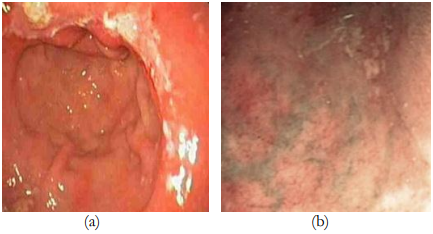
\includegraphics[width=0.5\textwidth]{images/wli-nbi.png}\\
  \label{fig:imageReal}
  \sourcecitation{\cite{rondonotti2015obscure}}
\end{figure}

O sensor complementa o sistema de iluminação através de mecanismos automáticos de controle de exposição (AEC) e ganho (AGC), que ajustam dinamicamente o tempo de integração e a amplificação do sinal para compensar variações de brilho. Essa combinação entre controle dos LEDs e recursos internos do sensor permite manter a qualidade da imagem ao mesmo tempo em que otimiza o consumo energético, aspecto crítico em dispositivos miniaturizados alimentados por bateria ou por transferência de energia sem fio.


\section{Processamento embarcado}

Esta seção aborda as principais restrições de hardware e a arquitetura de software típicas para sistemas embarcados de captura e transmissão de imagens em dispositivos com recursos limitados.

\subsection{Restrições de hardware em sistemas embarcados}

Projetos embarcados são fortemente condicionados por três variáveis: capacidade de processamento (frequência e arquitetura), memória volátil (RAM) e memória não volátil (flash), além do consumo energético associado. Microcontroladores de 8 bits apresentam tipicamente poucas dezenas de kilobytes de RAM, o que torna inviável o armazenamento de quadros inteiros. Por outro lado, plataformas ARM Cortex-M ou RP2040 oferecem mais memória e permitem estratégias de buffering mais elaboradas, facilitando a implementação de algoritmos de compressão moderadamente complexos. A escolha do microcontrolador deve, portanto, ser feita em função do balanço entre capacidade de cálculo necessária, disponibilidade de RAM para buffering e o orçamento energético do sistema \cite{armCortexM3TRM,rp2040Datasheet}.

Adicionalmente, a topologia de energia e a possibilidade de operar o processador em modos de baixo consumo entre eventos de aquisição influenciam a estratégia de processamento: algoritmos que demandam longos períodos de CPU a plena carga podem reduzir a autonomia mais que técnicas incrementais que processam os dados linha a linha com picos curtos de atividade.

\subsection{Arquitetura de software: fluxo de dados}

O fluxo de software típico em sistemas de captura e transmissão embarcada segue a cadeia aquisição → extração/pré-processamento → empacotamento → transmissão. Para operar com RAM reduzida, recomenda-se um processamento em streaming: cada linha recebida é pré-processada (por exemplo, extração de luminância, quantização ou compressão simples), empacotada em blocos compatíveis com o enlace e enviada antes que a linha seguinte seja completamente adquirida. Essa abordagem minimiza a necessidade de bufferização e permite que captura e transmissão ocorram em pipeline, exigindo mecanismos de sincronização no firmware que garantam determinismo temporal diante de interrupções e latências de periféricos (SPI/UART). Implementações robustas frequentemente adotam máquinas de estado simples para controlar a leitura, configuração e transmissão, priorizando previsibilidade sobre complexidade \cite{cavallotti2011fpga}.

\section{Compressão de imagens para transmissão embarcada}

Apresentam-se aqui os princípios e as métricas de avaliação relevantes para a compressão em dispositivos embarcados, bem como os métodos de baixa complexidade recomendados para validação conceitual.

\subsection{Princípios e métricas de avaliação}

Para aplicações embarcadas, a seleção de técnicas de compressão é orientada por um conjunto de métricas complementares, incluindo a taxa de compressão (razão entre o tamanho dos dados comprimidos e o original), a taxa efetiva de transmissão, a latência por quadro, o custo computacional (em ciclos de CPU por pixel) e o custo energético (em Joules por quadro). Em aplicações médicas, acrescenta-se ainda a necessidade de preservação da informação clínica relevante: quando a perda de informação é aceitável, a qualidade pode ser avaliada por métricas objetivas de similaridade entre imagens, enquanto em cenários que exigem integridade total dos dados empregam-se métodos \textit{cavallotti2011fpga}, acompanhados de mecanismos de verificação de integridade, como códigos de redundância cíclica (CRC). Em ambientes com recursos restritos, algoritmos com complexidade linear, baixa exigência de memória e reduzido custo computacional por pixel tendem a ser preferidos, mesmo quando proporcionam ganhos de compressão moderados \textcite{cavallotti2011fpga}.% \cite{sayood2017introduction}.

\subsection{Métodos de baixa complexidade}

Entre os métodos de baixa complexidade, o Run-Length Encoding (RLE) destaca-se pela simplicidade operacional e pela adequação ao processamento em fluxo contínuo. O RLE codifica sequências consecutivas de pixels com o mesmo valor por meio de pares formados pelo nível de intensidade e pela quantidade de repetições, exigindo apenas operações de comparação e incremento de contadores. Em imagens que apresentam regiões relativamente homogêneas, condição recorrente em diversas áreas do trato gastrointestinal, são observadas reduções de dados tipicamente entre 20\% e 40\%. Em contrapartida, em cenas com elevado ruído ou grande variação de intensidade, o desempenho do RLE pode ser reduzido, podendo inclusive resultar em expansão do volume de dados. Ainda assim, sua implementação simples em microcontroladores de 8 e 16 bits, a característica \textit{lossless} e a possibilidade de operação linha a linha tornam o RLE uma escolha pragmática para provas de conceito \cite{kim2021capsule}.

De forma complementar, esquemas diferenciais simples, como a modulação diferencial por código de pulso (DPCM), reduzem a entropia ao representar apenas a diferença entre pixels adjacentes. Quando combinados com o RLE, esses métodos podem aumentar a eficiência da compressão em regiões de variação gradual, mantendo baixo o custo computacional. Além disso, preservam o processamento em pipeline e reduzem a exigência de memória, atributos relevantes para validação experimental em plataformas de hardware com recursos limitados.

\subsection{Métodos avançados e estado da arte}

Técnicas baseadas em transformadas (por exemplo JPEG) e codificadores modernos (HEVC, AV1) alcançam compressões muito superiores, mas demandam memória e ciclos de CPU substanciais, além de maior complexidade de software. JPEG-LS oferece uma alternativa lossless com custo menor que JPEG2000, porém ainda acima da simplicidade de RLE/DPCM. Para etapas posteriores do projeto, em que hardware mais potente esteja disponível, essas técnicas são recomendadas; para a fase de validação conceitual, prioriza-se a robustez e a previsibilidade de métodos simples  \textcite{cavallotti2011fpga}. % \cite{cavallotti2011fpga,sayood2017introduction}.

\section{Comunicação sem fio e protocolo de enlace}

Esta seção aborda as tecnologias RF relevantes para o contexto e descreve princípios práticos de enlace e empacotamento lógico aplicáveis ao experimento de validação.

\subsection{Tecnologias RF e operação do NRF24L01}

A escolha da faixa de frequência e do transceptor de rádio envolve compromissos entre penetração em tecido biológico, taxa de dados disponível, consumo energético e requisitos regulatórios. A banda MICS (402–405 MHz) foi especificamente definida para dispositivos médicos implantáveis e apresenta melhor penetração em tecido quando comparada a frequências mais elevadas, como 2.4 GHz. Em contrapartida, módulos comerciais operando em MICS tendem a oferecer taxas de dados mais limitadas e maior complexidade regulatória, o que dificulta sua adoção em protótipos experimentais e validações iniciais. Por esse motivo, em ambientes de bancada e provas de conceito, é comum o uso de transceptores na faixa de 2.4 GHz, mesmo reconhecendo que esta não é a faixa ideal para uma aplicação clínica definitiva.

Nesse contexto, o NRF24L01 foi adotado como plataforma prática de validação. O transceptor opera na faixa de 2.4 GHz e disponibiliza taxas configuráveis de 250 kbps, 1 Mbps e 2 Mbps, além de incorporar mecanismos internos de verificação por CRC, confirmação automática de recebimento (auto-ack) e retransmissão automática. Esses recursos reduzem significativamente a complexidade do firmware, permitindo concentrar o desenvolvimento na validação do fluxo de aquisição, empacotamento e reconstrução dos dados, o que o torna adequado para experimentos de curto alcance em espaço livre \cite{nordic2013,valdastri2008transmission}.

O NRF24L01+ permite um payload máximo de 32 bytes por pacote de dados. Esse valor refere-se exclusivamente à carga útil disponível para a aplicação, sendo acrescido de campos adicionais no nível físico e de enlace, como preâmbulo, endereço, campo de controle e CRC, que compõem o tamanho total do pacote transmitido pelo rádio. A limitação do payload define diretamente a granularidade de fragmentação dos dados de imagem. Para um quadro em escala de cinza de 320×240 pixels, totalizando 76.800 bytes, a transmissão requer aproximadamente 2.400 pacotes de payload máximo, desconsiderando o overhead lógico introduzido pela aplicação. Esse elevado número de pacotes influencia o desenho do protocolo de camada superior, tornando indispensáveis mecanismos eficientes de numeração, detecção de perdas e remontagem correta dos dados no receptor.

\subsection{Protocolo interno do NRF24L01 e mecanismos de validação}

O transceptor NRF24L01 implementa um protocolo interno de enlace voltado à confiabilidade em curtas distâncias, combinando verificação de integridade, confirmação automática e retransmissão por hardware. Cada pacote transmitido segue um formato fixo definido pelo próprio módulo, ilustrado na Figura \ref{fig:frame-protocolo}. O quadro é composto por um \textit{preamble} de 1 byte para sincronização, seguido por um campo de endereço configurável entre 3 e 5 bytes, um campo de controle do pacote (Packet Control Field, PCF), um \textit{payload} de até 32~bytes e, por fim, um CRC de 1 ou 2 bytes \cite{nordic2013}. O PCF contém informações essenciais para a lógica interna: o comprimento do payload, um identificador de pacote (PID) de 2bits e um \textit{No-Ack bit} opcional que suprime confirmações quando desejado.

\begin{figure}[htbp]
  \centering
  \caption{Estrutura do pacote RF do NRF24L01, contendo preâmbulo, endereço, campo de controle, payload e CRC.}
  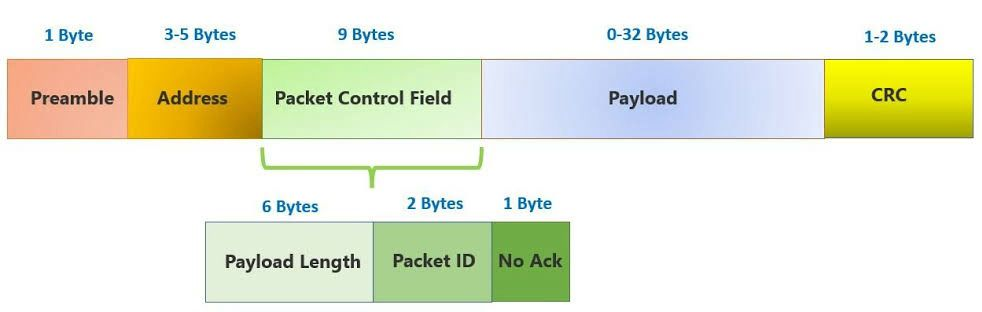
\includegraphics[width=0.85\textwidth]{images/frame.jpg}
  \label{fig:frame-protocolo}
  \sourcecitation{Adaptado de \cite{nordic2013}.}
\end{figure}

O PID é o principal mecanismo de detecção de duplicidade. A cada novo pacote enviado, o transceptor alterna ciclicamente o PID entre quatro valores possíveis. No receptor, pacotes recebidos com um PID repetido e mesmo conteúdo são automaticamente descartados como duplicatas, evitando reprocessamento quando retransmissões ocorrem. Após a recepção correta de um pacote, o módulo pode enviar automaticamente um ACK contendo um \textit{payload} opcional (quando habilitado), permitindo comunicação bidirecional com baixa sobrecarga \cite{nordic2013,valdastri2008transmission}. Caso o transmissor não receba o ACK dentro da janela definida, o NRF24L01 aciona o mecanismo de \textit{Auto-Retransmit}, reenviando o pacote até o limite programado.

O CRC protege o quadro contra erros de canal. O transmissor calcula o CRC sobre endereço, PCF e payload; o receptor valida esse valor e descarta automaticamente quadros corrompidos. Esses mecanismos garantem integridade local, porém não oferecem recursos de reordenação, controle de fluxo ou reconstrução de dados fragmentados , responsabilidades delegadas ao nível lógico da aplicação.

Assim, embora o protocolo interno do NRF24L01 assegure entrega confiável de pacotes individuais, a transmissão de quadros de imagem requer um protocolo de aplicação adicional capaz de numerar pacotes, agrupar fragmentos, identificar quadros completos e solicitar retransmissões seletivas quando necessário.

\section{Métricas e estratégias de validação experimental}

A validação experimental deve quantificar o comportamento do sistema sob condições controladas, variando parâmetros-chave de modo a produzir curvas de desempenho representativas. Neste trabalho, adotam-se métricas comumente empregadas na avaliação de sistemas de comunicação embarcados e transmissão de imagens, a saber: taxa efetiva de transferência (bits por segundo úteis), taxa de quadros entregues (FPS), percentual de pacotes recebidos com sucesso, latência média por quadro e consumo energético estimado por quadro transmitido. Essas métricas permitem caracterizar de forma objetiva tanto o desempenho do enlace quanto o impacto das escolhas de projeto adotadas.

A coleta sistemática dessas grandezas em função de variáveis controláveis, como distância entre transmissor e receptor, potência de transmissão configurada, presença de elementos atenuadores representativos de tecido e uso ou não de compressão, possibilita avaliar a robustez do enlace e a eficácia das técnicas empregadas. Em particular, a comparação direta entre cenários com e sem compressão, como no caso do RLE, evidencia o compromisso entre aumento de throughput, custo computacional adicional e impacto energético, fornecendo subsídios técnicos para recomendações e extensões futuras do projeto.

Em síntese, a fundamentação apresentada fornece base técnica suficiente para sustentar as decisões experimentais adotadas ao longo do trabalho. As restrições energéticas e de memória delimitam o espaço de soluções viáveis, enquanto sensores CMOS com interface DVP impõem requisitos temporais rigorosos ao firmware. Nesse contexto, técnicas de compressão simples e processamento em streaming, como RLE e DPCM, mostram-se adequadas para validações iniciais. Adicionalmente, o NRF24L01 constitui uma plataforma prática para testes de enlace, oferecendo mecanismos de confiabilidade integrados que facilitam a avaliação experimental. Essas diretrizes orientam diretamente as implementações e os testes descritos nas seções experimentais subsequentes.


% Observação final: referencias bibliográficas devem estar presentes no .bib do projeto.
% Use as chaves citadas: motta2016transmissao, murliky2017multivariable, basar2014application, meng2021novel,
% cavallotti2011fpga, gao2022stable, kim2021capsule, valdastri2008transmission, nordic2013, sayood2017introduction, zhang2024transmitter, armCortexM3TRM, rp2040Datasheet, etc.




%%%%%%%%%%%%%%%%%%%%%%%%%%%%%%%%%%%%%%%%%%%%%%%%%%%%%%%%%%%%%%
%%%%%%%%%%%%%%%%%%%%%%%%%%%%%%%%%%%%%%%%%%%%%%%%%%%%%%%%%%%%%%
%%%%%%%%%%%%%%% METODOLOGIA E IMPLEMENTACAO DOS RESULTADOS %%%%%%%%%%%%%%%
%%%%%%%%%%%%%%%%%%%%%%%%%%%%%%%%%%%%%%%%%%%%%%%%%%%%%%%%%%%%%%
%%%%%%%%%%%%%%%%%%%%%%%%%%%%%%%%%%%%%%%%%%%%%%%%%%%%%%%%%%%%%%
\chapter{Metodologia Adotada}

Este capítulo descreve minuciosamente a implementação prática do sistema proposto, enfatizando as decisões de projeto, os procedimentos executados para integrar hardware e software e as metodologias adotadas na validação experimental. Todo o código-fonte desenvolvido no contexto deste trabalho, incluindo firmware dos microcontroladores e aplicações de apoio para recepção e reconstrução das imagens, encontra-se disponível publicamente em \url{github.com/MottaGit/tcc-leonardo-motta-engenharia-controle-automacao}. O objetivo deste capítulo é demonstrar como o protótipo foi estruturado e avaliado, permitindo compreender tanto o funcionamento interno da solução quanto a confiabilidade dos resultados obtidos. São apresentadas a arquitetura geral, a definição do hardware, o sistema de software desenvolvido e a análise detalhada das quatro etapas de testes realizadas.


\section{Arquitetura proposta}

A arquitetura concebida tem como finalidade validar, em ambiente controlado de bancada, os principais subsistemas eletrônicos que compõem uma cápsula endoscópica sem fio, em especial o fluxo completo de aquisição de imagens, empacotamento, transmissão sem fio, recepção e reconstrução dos quadros. Embora a implementação não tenha como foco a miniaturização física do sistema, as escolhas arquiteturais foram guiadas pelos mesmos tipos de restrições presentes na aplicação real, como limitações de processamento, memória, largura de banda e consumo energético. Dessa forma, o protótipo desenvolvido representa funcionalmente o comportamento esperado de uma cápsula endoscópica, permitindo avaliar a viabilidade técnica das soluções adotadas antes de uma futura integração em escala reduzida.

O módulo transmissor foi implementado com um Arduino Mega 2560, utilizado como plataforma de desenvolvimento para representar a unidade de processamento embarcada da cápsula. A escolha do Mega se deve à sua maior capacidade de memória e à disponibilidade de portas digitais suficientes para operar o barramento paralelo de 8 bits da câmera OV7670, condição necessária para a leitura síncrona dos dados de imagem. O microcontrolador dispõe de 256~kB de memória Flash e 8~kB de SRAM, recursos que possibilitam o armazenamento de buffers intermediários e o controle do fluxo de transmissão de pacotes. Embora esse microcontrolador não seja adequado para algoritmos avançados de compressão, sua utilização é coerente com o objetivo de validar o encadeamento funcional da aquisição e transmissão de dados, de forma análoga ao que ocorreria em um sistema embarcado de cápsula endoscópica.

A câmera OV7670 foi configurada para operar no formato YUV422, utilizando exclusivamente o componente de luminância (Y), o que reduz o volume de dados transmitidos para metade em relação ao formato RGB565. Essa escolha está alinhada com aplicações de cápsula endoscópica, nas quais a informação estrutural da imagem é prioritária e a redução de dados impacta diretamente a taxa de quadros e o consumo energético. O uso de barramento paralelo e sinais dedicados de sincronismo impõe requisitos temporais rigorosos ao firmware, justificando a necessidade de um microcontrolador com maior flexibilidade para tratamento de interrupções e leitura síncrona.

A transmissão sem fio foi implementada com o módulo NRF24L01+, que opera na faixa de 2,4~GHz e incorpora mecanismos nativos de confiabilidade, como verificação por CRC, confirmação automática de recebimento e buffers FIFO. Esses recursos permitem reproduzir, em escala experimental, o comportamento de um enlace sem fio confiável para transmissão de imagens a curta distância, cenário compatível com a comunicação entre uma cápsula endoscópica e um receptor externo posicionado próximo ao corpo do paciente. O payload máximo de 32 bytes por pacote impõe fragmentação dos quadros, característica que influencia diretamente o desenho do protocolo lógico avaliado neste trabalho.

Em relação ao consumo, embora não tenha sido realizada uma análise energética completa, os valores típicos de corrente do transceptor e dos demais componentes foram considerados apenas como referência de viabilidade. A compatibilidade mencionada refere-se ao fato de que os níveis de potência envolvidos estão na mesma ordem de grandeza daqueles encontrados em sistemas embarcados alimentados por bateria ou por transmissão de energia sem fio, não implicando inviabilidade conceitual do uso desses subsistemas em uma cápsula endoscópica real.

O receptor foi implementado com um Arduino Uno, cuja função é representar a unidade externa de coleta de dados. Sua capacidade é suficiente para receber os pacotes transmitidos, realizar validações básicas e encaminhar os dados ao computador por meio da interface UART. A reconstrução completa dos quadros é realizada no computador, reduzindo a carga computacional do receptor embarcado e refletindo uma arquitetura típica de cápsula endoscópica, na qual o processamento mais pesado é deslocado para o sistema externo.

\section{Definição do hardware}

O hardware foi integrado em bancada utilizando cabos curtos e conexões diretas, o que reduziu interferências eletromagnéticas e garantiu estabilidade nos testes. A alimentação foi fornecida por fonte regulada de 5 V, com conversão local para 3,3 V quando necessário. A Figura \ref{fig:hardware-diagramal} apresenta o diagrama geral de interligação.

\begin{figure}[htbp]
  \centering
  \caption{Diagrama esquemático da arquitetura de hardware proposta, conexões para a câmera (a esquerda), conexões para o módulo transmissor (a direita).}
  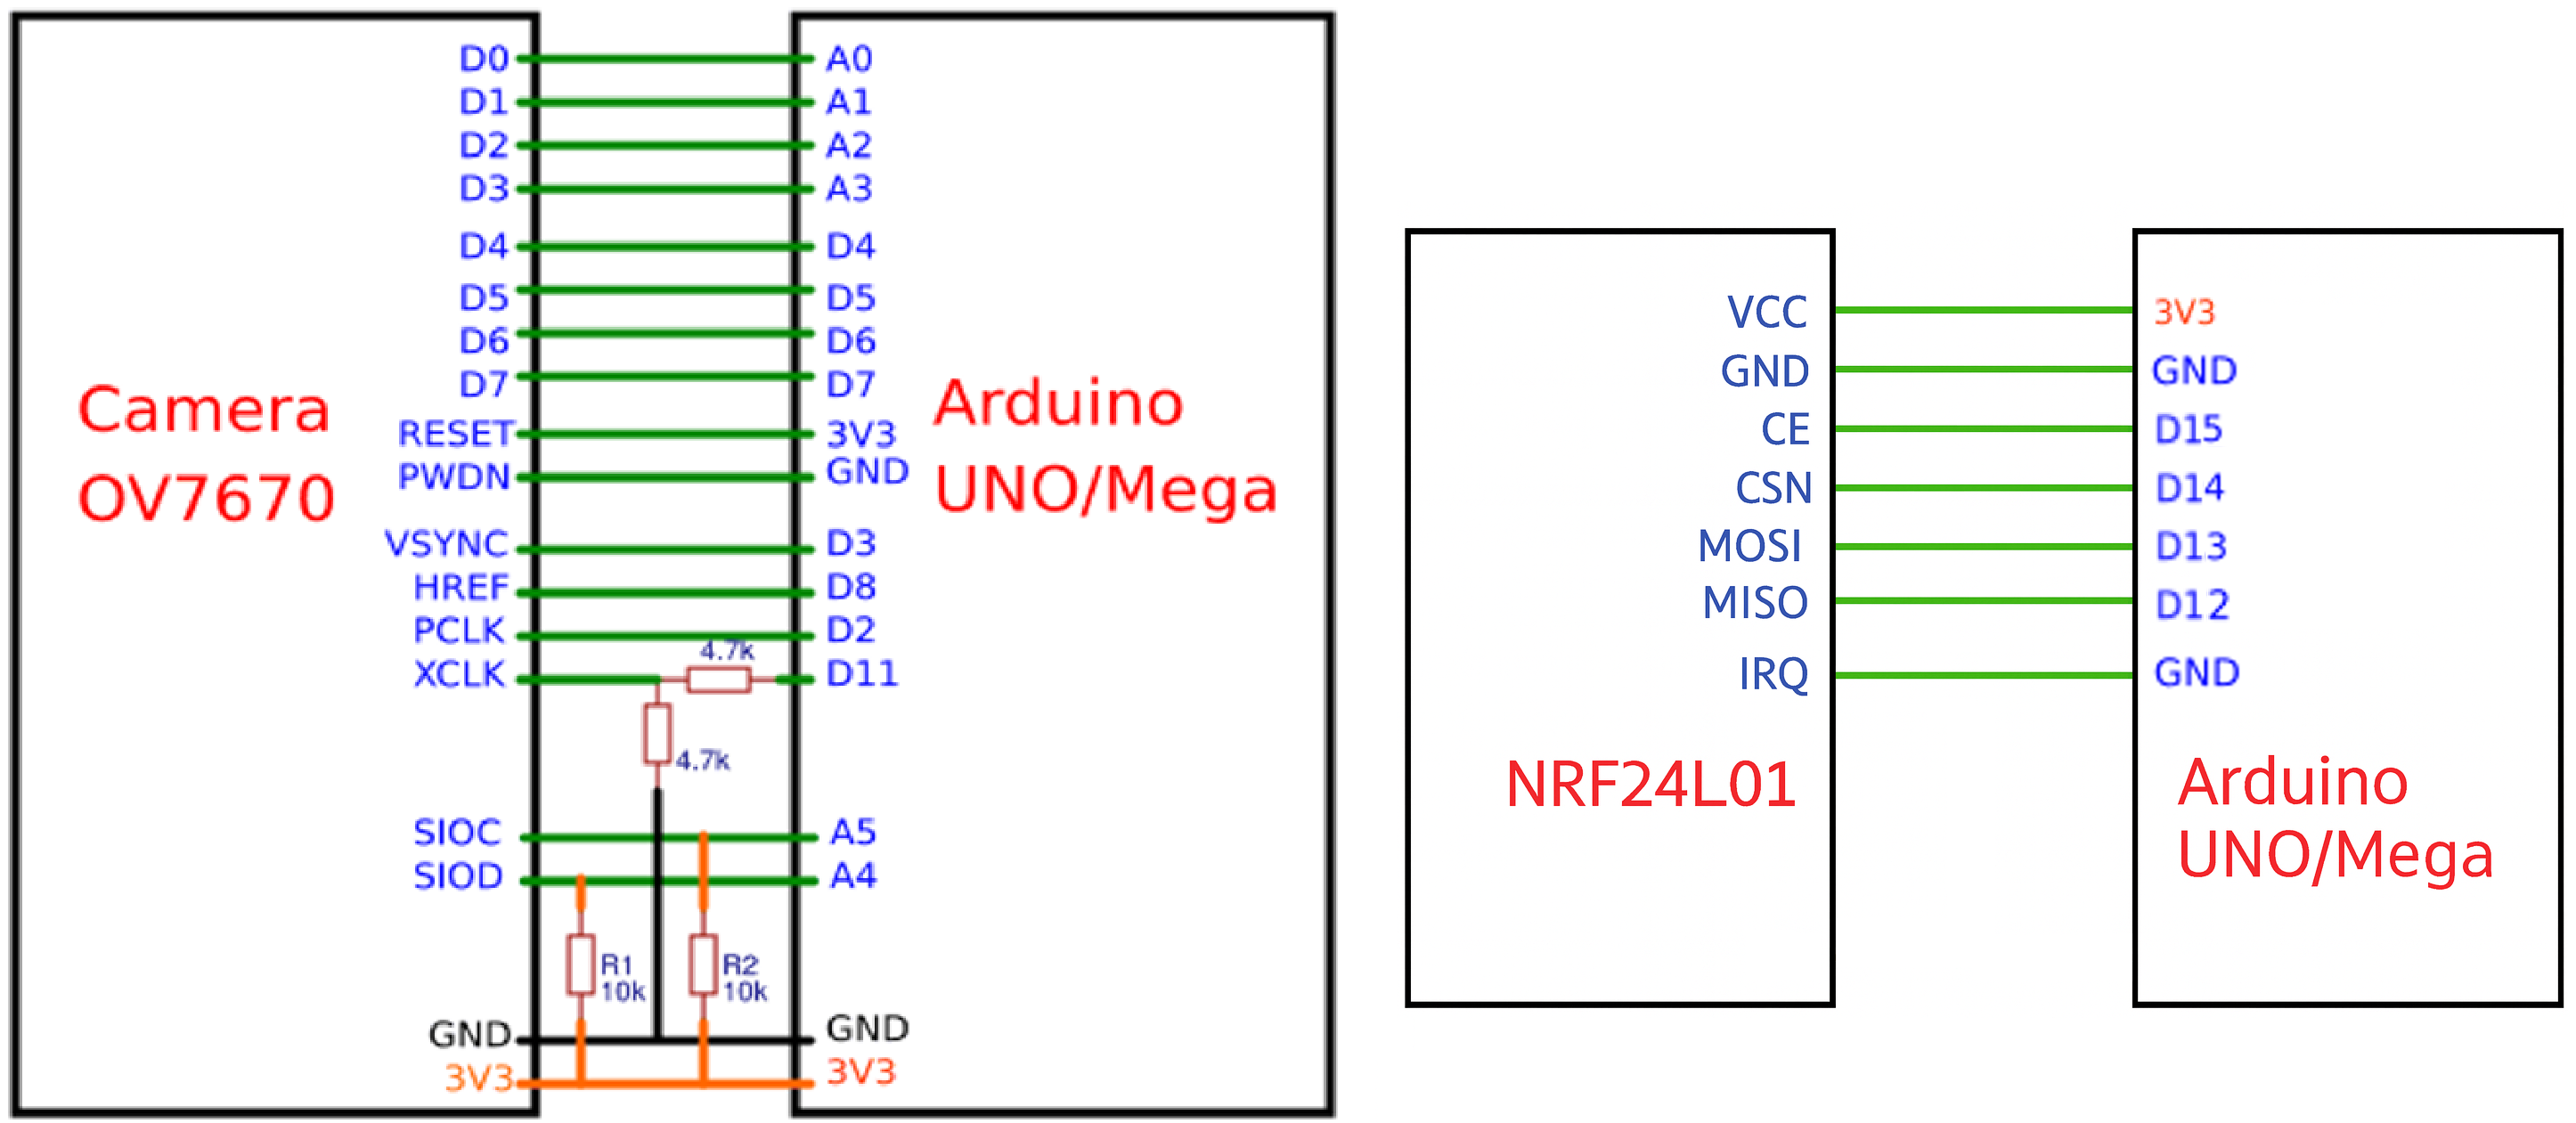
\includegraphics[width=0.6\textwidth]{images/hardware.png}\\
  \label{fig:hardware-diagramal}
  \sourcecitation{Elaborado pelo autor (2025).}
\end{figure}

O barramento paralelo da OV7670 foi conectado diretamente aos pinos digitais do Mega, preservando sinais essenciais como VSYNC, HREF e PCLK. As linhas do barramento I2C receberam resistores de pull-up de 10 k\(\Omega\). O sinal de clock da câmera exigiu redução para nível de 3,3 V por divisor resistivo. Para o NRF24L01+, capacitores de desacoplamento de 10 µF e 100 nF foram posicionados próximos ao módulo para garantir estabilidade da alimentação. A conexão SPI foi mantida com cabos curtos para evitar instabilidade.

Essa estrutura foi projetada para permitir substituição futura do microcontrolador por modelos mais potentes, bem como a inserção de módulos adicionais, como um acelerador de compressão.

\section{Sistema de software}

O software do protótipo foi desenvolvido em C na IDE Arduino, com organização modular para facilitar manutenção e expansão. As etapas de aquisição e transmissão foram implementadas no transmissor, enquanto a recepção e reconstrução dos quadros ficaram divididas entre o Arduino Uno e o computador. A comunicação com o PC foi realizada em Python no transmissor e em Java no monitor serial do receptor.

\subsection{Protocolo de comunicação}

O protocolo implementado respeita as limitações do NRF24L01+ e aproveita suas funções internas de confiabilidade. Cada pacote possui 32 bytes, sendo 4 para o cabeçalho e 28 para os dados da imagem. O cabeçalho inclui sinalização de início e fim de quadro, início e fim de linha, número de sequência (12 bits), identificador de quadro e um CRC-8 lógico calculado apenas sobre o payload. Mesmo com o CRC físico do transceptor, o CRC lógico possibilita verificar corrupção específica do conteúdo da imagem.

Pacotes fora de ordem são reagrupados conforme o número de sequência. Pacotes duplicados são ignorados, e pacotes faltantes são marcados como vazios para fins de depuração. Essa estrutura mostrou-se suficiente para garantir integridade e rastreamento dos quadros.

\subsection{Câmera}

A configuração da OV7670 foi realizada com escrita de registradores via I2C. A resolução foi ajustada para 320×240 pixels, e o clock para 8 MHz. Filtros automáticos foram desativados para evitar interferências no processo de validação. O controle automático de ganho e exposição foi mantido, adequado ao ambiente de bancada.

\subsection{Fluxo de código}

\subsubsection{Fluxo de transmissão}

O transmissor inicia configurando a câmera, o barramento I2C e o NRF24L01+. Em seguida, entra em laço contínuo. A cada ativação de VSYNC, um novo quadro é iniciado. O microcontrolador lê cada byte conforme o ritmo ditado pelo PCLK, armazenando temporariamente os dados em memória.

A montagem dos pacotes ocorre simultaneamente à captura. Assim que 28 bytes de imagem são acumulados, o pacote é finalizado com o cabeçalho e enviado via SPI ao NRF24L01+, que realiza retransmissões automáticas e confirmação de entrega. Esse processo se repete até o fim do quadro, quando o contador de frame é incrementado.

\begin{figure}[htbp]
  \centering
  \caption{Fluxograma do código de transmissão implementado no microcontrolador.}
  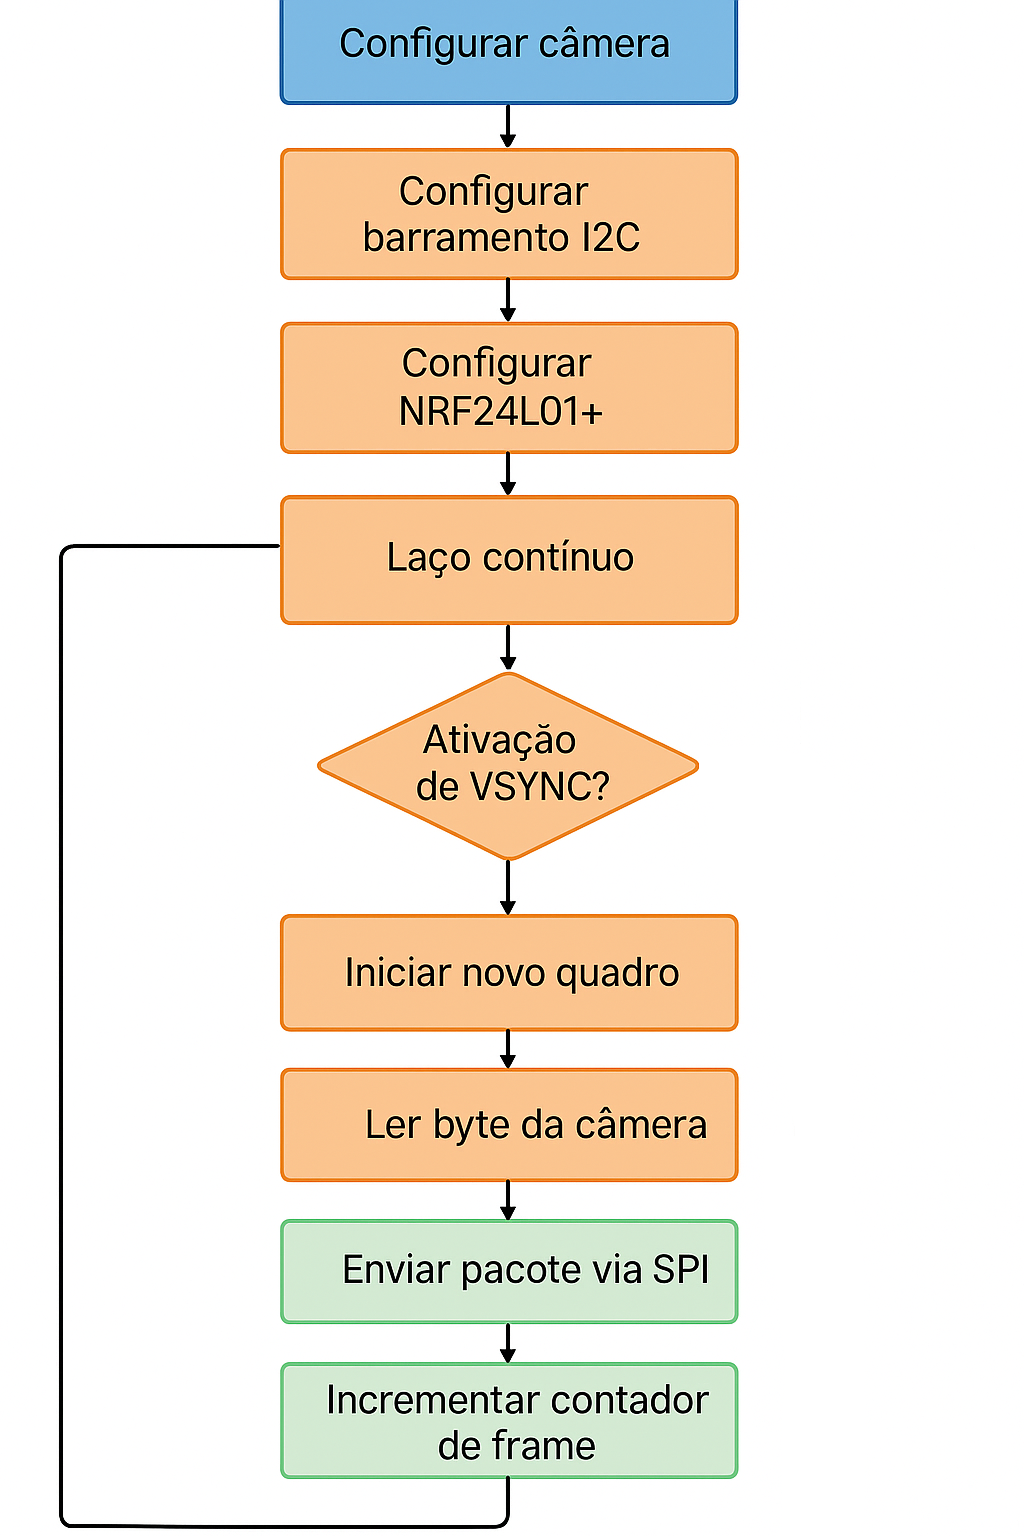
\includegraphics[width=0.3\textwidth]{images/fluxo.png}\\
  \label{fig:fluxo-codigo}
  \sourcecitation{Elaborado pelo autor (2025).}
\end{figure}

\subsubsection{Fluxo de recepção e reconstrução}

O receptor inicia configurando o módulo NRF24L01+ para modo de escuta. Sempre que um pacote é recebido, o Uno valida o CRC físico e encaminha o pacote diretamente pela UART ao computador. Não há processamento local além da verificação de integridade básica.

No computador, um programa em Java lê os pacotes, reorganiza-os com base no número de sequência e monta o quadro completo. Pacotes ausentes são registrados, e quadros incompletos são exibidos para depuração. Ao final da montagem, o quadro é salvo em formato PNG.

\section{Testes e resultados obtidos}

As medições foram realizadas em quatro etapas experimentais. Em todas as fases, foram registradas as métricas de tempo, taxa de quadros, perda de pacotes, retransmissões, consumo elétrico e qualidade visual das imagens.

\subsection{Etapa 1: transmissão de dados brutos via serial}

A primeira etapa experimental teve como objetivo validar o processo de aquisição de imagem e a integridade dos dados provenientes da câmera OV7670, isolando completamente o sistema de comunicação sem fio e qualquer lógica adicional de empacotamento. Nessa fase, buscou-se verificar se o microcontrolador era capaz de ler corretamente o barramento paralelo da câmera e transferir os dados ao computador sem perdas, inversões de bytes ou erros de sincronismo.

O Arduino Mega 2560 capturou quadros completos da OV7670 configurada em modo YUV422, utilizando apenas o componente de luminância (Y), resultando em imagens em tons de cinza com resolução de 320×240 pixels. Cada quadro, totalizando 76.800 bytes, foi transmitido sequencialmente ao computador por meio da interface UART, sem qualquer tipo de fragmentação, cabeçalho ou compressão. O tempo de transmissão por quadro foi medido utilizando contadores internos do microcontrolador e confirmado por medições externas, resultando em um valor médio de aproximadamente 1,55 s por quadro, o que evidencia que a taxa da interface serial foi o principal fator limitante do desempenho nesta etapa.

As imagens reconstruídas no computador apresentaram elevada integridade visual, com correta organização espacial dos pixels e ausência de artefatos significativos. A Figura \ref{fig:test-serial-frame}, à esquerda, ilustra um quadro típico reconstruído a partir da transmissão direta dos dados brutos, demonstrando que a cadeia de captura e leitura do barramento paralelo da câmera operou de forma consistente. Essa etapa confirmou a confiabilidade do pipeline básico de aquisição, servindo como referência para as etapas subsequentes de validação do protocolo lógico.

\begin{figure}[htbp]
  \centering
  \caption{Na esquerda exemplo de imagem reconstruída via transmissão serial direta, na direita exemplo de imagem reconstruída com glitches.}
  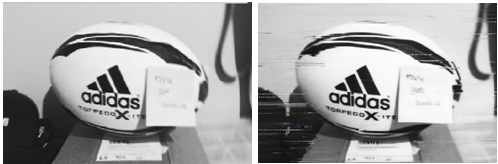
\includegraphics[width=0.8\textwidth]{images/exemplo.png}\\
  \label{fig:test-serial-frame}
  \sourcecitation{Elaborado pelo autor (2025).}
\end{figure}

\subsection{Etapa 2: validação do protocolo lógico}

Com a aquisição básica validada, a segunda etapa concentrou-se na verificação do protocolo lógico de empacotamento e reconstrução dos dados, mantendo ainda a transmissão via UART para eliminar variáveis associadas ao enlace sem fio. O objetivo foi avaliar o impacto da fragmentação dos quadros em pacotes, da inclusão de cabeçalhos e da reorganização dos dados no receptor.

Nesta fase, os quadros capturados foram segmentados em pacotes contendo cabeçalho lógico e payload de dados, conforme definido no protocolo do sistema. O receptor emulou o comportamento esperado para a comunicação RF, realizando a leitura sequencial dos pacotes, a validação do CRC lógico e a reconstrução da imagem com base no número de sequência e nos marcadores de início e fim de quadro. Para avaliar a robustez do protocolo, foram inseridas artificialmente perdas de pacotes e alterações na ordem de entrega durante a transmissão serial.

Os testes demonstraram que o protocolo foi capaz de detectar corretamente pacotes ausentes e manter a coerência estrutural do quadro. Quando até 5\% dos pacotes eram removidos, a imagem ainda podia ser reconstruída, embora com falhas visuais localizadas. Essas falhas manifestaram-se principalmente como linhas horizontais incompletas ou regiões com ausência de pixels, fenômeno visível na Figura \ref{fig:test-serial-frame}, à direita, onde são observados \textit{glitches} associados à perda de pacotes durante o empacotamento. Ainda assim, a organização global da imagem foi preservada, evidenciando que a numeração de pacotes e os campos de controle foram eficazes para reordenar os dados mesmo em cenários de entrega fora de ordem.

Essa etapa confirmou que a lógica de empacotamento e reconstrução funciona conforme o esperado e que o sistema é capaz de lidar com falhas pontuais de transmissão, preparando o terreno para a introdução do enlace sem fio na etapa seguinte.

\subsection{Etapa 3: transmissão sem fio via NRF24L01+}

A terceira etapa experimental introduziu o enlace sem fio no sistema, com o objetivo de avaliar o desempenho da transmissão de quadros de imagem completos utilizando os módulos NRF24L01+. Diferentemente das etapas anteriores, nesta fase o sistema operou com todas as camadas previstas no projeto: aquisição, empacotamento lógico, transmissão RF, recepção, reorganização dos pacotes e reconstrução da imagem no computador.

A comunicação sem fio foi configurada para operar a uma taxa nominal de 1 Mbps, valor escolhido como compromisso entre confiabilidade e vazão efetiva. Cada quadro de imagem em tons de cinza, com resolução de 320×240 pixels, foi fragmentado em aproximadamente 2.740 pacotes, considerando o payload máximo de 32 bytes por transmissão. Durante os testes, foram registradas métricas como o tempo total de transmissão por quadro (obtido por meio de timestamps no transmissor e no computador), a taxa de sucesso na entrega dos pacotes (relação entre pacotes esperados e recebidos), o número de retransmissões automáticas realizadas pelo transceptor e o consumo elétrico do sistema, medido com multímetro em série com a alimentação.

\begin{figure}[htbp]
  \centering
  \caption{Montagem experimental da transmissão sem fio com módulos NRF24L01+.}
  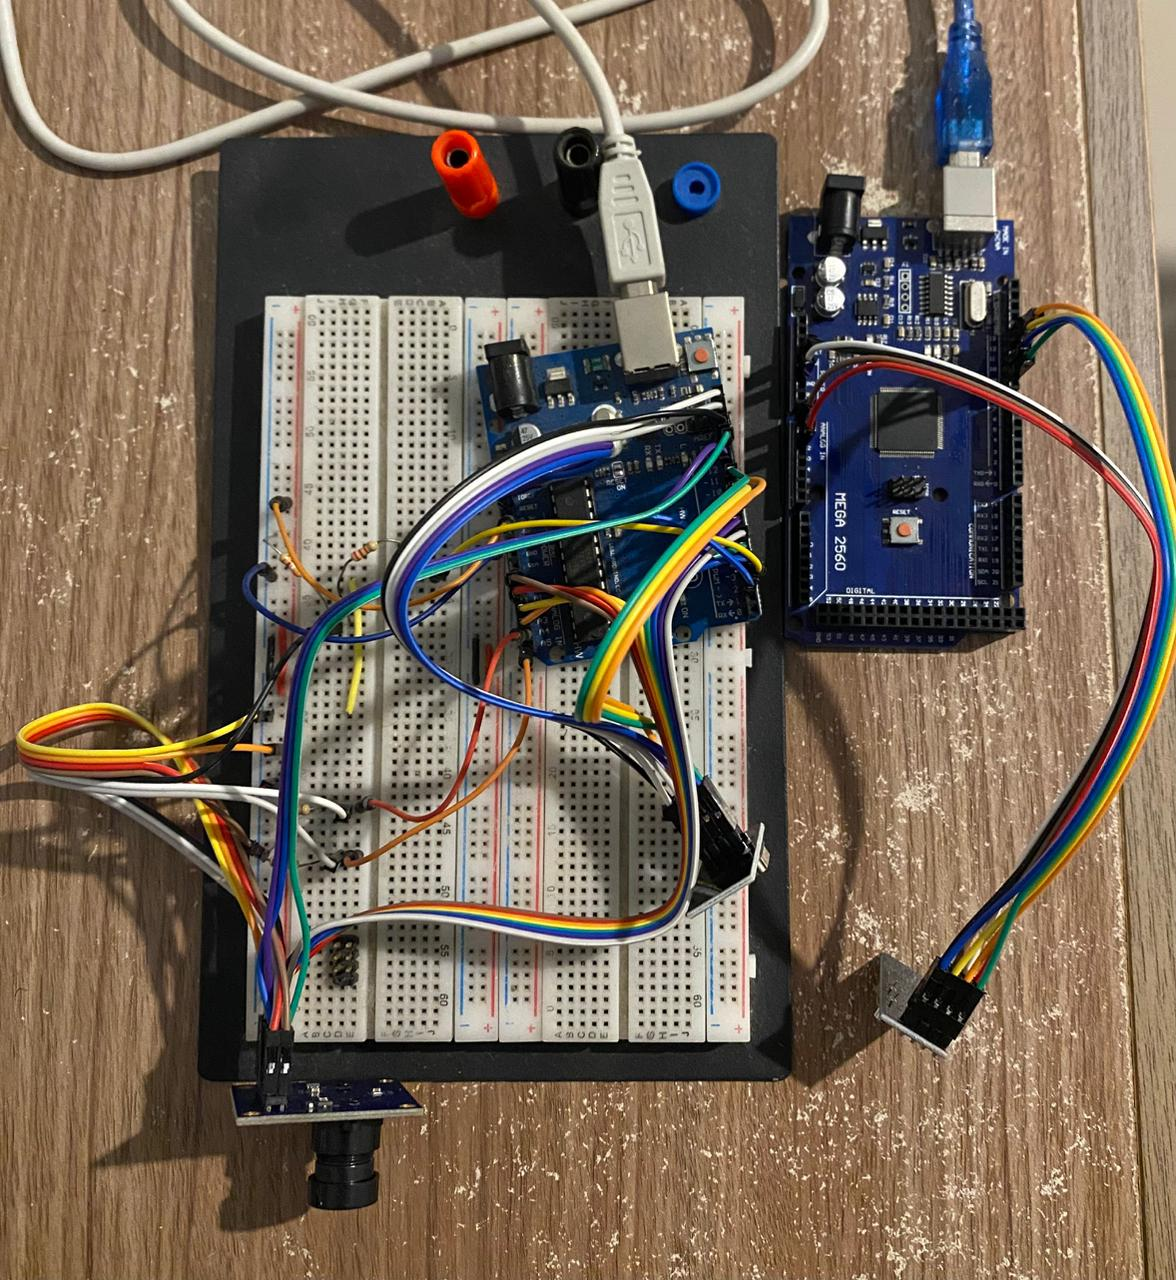
\includegraphics[width=0.45\textwidth]{images/montagem-prototipo.png}\\
  \label{fig:teste-transmissao}
  \sourcecitation{Elaborado pelo autor (2025).}
\end{figure}

Os experimentos foram conduzidos em ambiente de bancada, com distância inicial de aproximadamente 1 metro entre transmissor e receptor, sendo posteriormente estendida até 3 metros. Os resultados indicaram uma taxa média de sucesso de entrega de 97,4\% a 1 metro e 94,1\% a 3 metros, demonstrando boa robustez do enlace em condições de linha de visada. As imagens reconstruídas mantiveram estabilidade visual, com falhas pontuais associadas principalmente à perda de pacotes, mas sem comprometer a interpretação geral do quadro.

A Figura \ref{fig:teste-transmissao} ilustra a montagem experimental adotada nesta etapa, evidenciando a disposição física dos módulos, do microcontrolador transmissor, do receptor e do computador responsável pela reconstrução das imagens. A principal limitação observada nesta fase foi a largura de banda efetiva do enlace RF, que impôs restrições diretas à taxa de quadros alcançável, mesmo com os mecanismos automáticos de retransmissão do módulo.

\subsection{Etapa 4: implementação e teste do algoritmo de compressão RLE}

A quarta etapa teve como objetivo avaliar o impacto da aplicação de um algoritmo de compressão simples sobre o desempenho global do sistema de transmissão. Para isso, foi implementado o algoritmo Run-Length Encoding (RLE) diretamente no fluxo de dados do transmissor, antes do empacotamento e envio dos pacotes via RF. O RLE foi escolhido por sua baixa complexidade computacional, operação \textit{lossless} e compatibilidade com microcontroladores de recursos limitados.

O algoritmo atua agrupando sequências consecutivas de pixels com o mesmo valor de intensidade em pares do tipo (valor, comprimento), reduzindo o volume total de dados a serem transmitidos, especialmente em regiões visualmente homogêneas. A descompressão foi realizada no lado do receptor, antes da reconstrução final da imagem. Os testes mostraram que a eficiência do RLE depende fortemente do conteúdo visual da cena: em imagens com grandes áreas uniformes, a taxa de compressão variou entre 30\% e 40\%, enquanto em cenas mais ruidosas ou com alto nível de detalhe os ganhos foram mais modestos, em torno de 15\%.

A Tabela \ref{tab:rle-resultados} resume quantitativamente os principais resultados obtidos com e sem o uso de compressão. Observa-se uma redução média de 34,4\% no tamanho dos quadros, acompanhada de um aumento significativo na taxa de quadros transmitidos, que passou de 1,25 FPS para aproximadamente 1,98 FPS. O tempo médio de transmissão por quadro também foi reduzido em cerca de 31\%, evidenciando o impacto direto da compressão na vazão efetiva do sistema. A taxa de sucesso de pacotes apresentou leve redução, inferior a 1\%, atribuída ao aumento da variabilidade no tamanho dos pacotes, mas sem comprometer a estabilidade geral do enlace.

\begin{table}[!htbp]
\centering
\caption{Resultados médios da transmissão com e sem compressão.}
\label{tab:rle-resultados}
\begin{tabular}{|l|c|c|c|}
\hline
\textbf{Parâmetro} & \textbf{Sem compressão} & \textbf{Com RLE} & \textbf{Ganho (\%)} \\ \hline
Tamanho médio por quadro (bytes) & 76.800 & 50.400 & 34,4 \\ \hline
Taxa média de quadros (FPS) & 1,25 & 1.98 & 50,8 \\ \hline
Taxa de sucesso de pacotes (\%) & 97,4 & 96,8 & -0,6 \\ \hline
Tempo médio de transmissão (s) & 0,80 & 0,56 & 31 \\ \hline
\end{tabular}
\end{table}

\subsection{Análise consolidada dos resultados}

A análise conjunta das quatro etapas experimentais confirma que o sistema desenvolvido atende plenamente aos objetivos de validação conceitual propostos. A etapa inicial demonstrou a confiabilidade do processo de aquisição e leitura dos dados da câmera CMOS, enquanto a validação do protocolo lógico evidenciou a capacidade do sistema de detectar perdas, reorganizar pacotes e manter a coerência estrutural das imagens. A introdução do enlace sem fio mostrou que o NRF24L01+ é capaz de sustentar a transmissão de quadros completos com taxas de sucesso superiores a 94\% em condições controladas, ainda que limitado pela largura de banda disponível.

A aplicação do algoritmo de compressão RLE revelou-se eficaz para melhorar o desempenho do sistema, proporcionando aumento significativo da taxa de quadros e redução do tempo de transmissão sem deteriorar de forma relevante a qualidade visual das imagens. A Figura \ref{fig:comparativo-resultados} apresenta um comparativo visual entre imagens transmitidas sem compressão e com compressão RLE, evidenciando que, apesar de pequenas variações locais, a estrutura global e a legibilidade dos quadros foram preservadas.

\begin{figure}[htbp]
  \centering
 \caption{Comparativo entre imagens transmitidas sem compressão (esquerda) e com compressão RLE (direita).}
  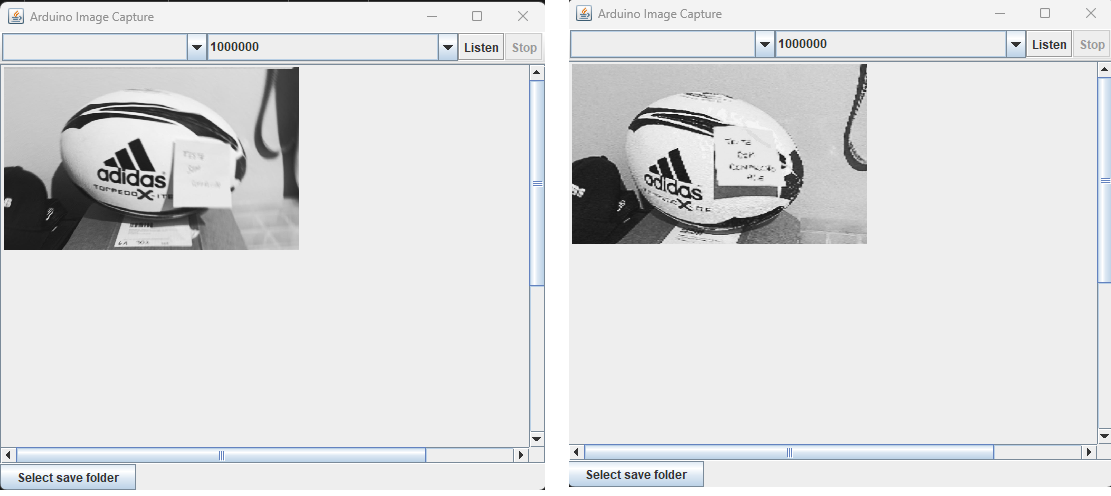
\includegraphics[width=0.8\textwidth]{images/comparativo.png}\\
 \label{fig:comparativo-resultados}
  \sourcecitation{Elaborado pelo autor (2025).}
\end{figure}

Em síntese, a prova de conceito pode ser considerada bem-sucedida. O sistema apresentou operação estável, baixo índice de erro, desempenho compatível com os recursos empregados e resultados coerentes com as expectativas teóricas. Esses resultados estabelecem uma base sólida para evoluções futuras, como a adoção de microcontroladores mais potentes e a implementação de algoritmos de compressão mais eficientes.






%%%%%%%%%%%%%%%%%%%%%%%%%%%%%%%%%%%%%%%%%%%%%%%%%%%%%%%%%%
%%%%%%%%%%%%%%%%%%%% CONLUSOES %%%%%%%%%%%%%%%%%%%%%%%%%%%%%%
%%%%%%%%%%%%%%%%%%%%%%%%%%%%%%%%%%%%%%%%%%%%%%%%%%%%%%%%%%


\chapter{Conclusões e Trabalhos Futuros}

Os resultados obtidos demonstram que o sistema desenvolvido para captura, empacotamento, transmissão e reconstrução de imagens utilizando o transceptor NRF24L01+ operou de forma consistente e adequada aos objetivos de validação conceitual. A transmissão de quadros grayscale em resolução QVGA resultou em aproximadamente 76.800 bytes por imagem, exigindo cerca de 2.743 pacotes por quadro devido ao limite de 28 bytes úteis por pacote. Na configuração sem compressão, observou-se tempo médio de 1,58 segundos por quadro (0,63 FPS) e taxa de sucesso de pacotes de 97,4\%. Com a compressão RLE, o tamanho médio por quadro reduziu-se para cerca de 50.400 bytes, elevando a taxa de quadros para aproximadamente 0,95 FPS e mantendo alta confiabilidade de entrega (96,8\%). Esses dados demonstram que o pipeline completo funcionou de forma estável, com imagens reconstruídas satisfatórias e desempenho coerente com as limitações do hardware empregado.

A validação confirma que a arquitetura proposta cumpre sua finalidade: estabelecer, com precisão e de maneira mensurável, a viabilidade técnica de um enlace de transmissão de imagem baseado em hardware acessível. O sistema mostrou integridade na captura, previsibilidade na camada lógica e estabilidade no enlace RF, constituindo uma base sólida para desenvolvimento posterior.

Apesar dos resultados positivos, os testes também evidenciaram limitações inerentes à plataforma utilizada, principalmente no que diz respeito à largura de banda disponível e à ausência de capacidade de compressão mais avançada no microcontrolador. Como próximos passos, torna-se necessário evoluir em três eixos principais: adoção de algoritmos de compressão mais eficientes (como JPEG-LS, DPCM otimizado ou esquemas wavelet leves), implementação em microcontroladores mais potentes (por exemplo, ARM Cortex-M4/M7) capazes de executar compressão em tempo real e manter buffers maiores, e aprimoramento do protocolo de comunicação para aumentar robustez e eficiência.

Etapas futuras também devem considerar maior integração física, estudo energético mais detalhado, otimização de antenas e posterior acoplamento com o sistema de transferência de energia sem fio da cápsula endoscópica. Com isso, o trabalho avança como uma etapa intermediária importante na construção de um protótipo funcional, delineando com clareza os resultados já alcançados e as direções necessárias para uma solução mais completa e próxima das demandas clínicas reais.



\printbibliography

\end{document}

